\chapter{同伦类型论}
\section{K原理的独立性}\label{hott:independent}
我们刚才已经看到相等类型的归纳子, 也就是 J 原理. 它直觉上大致说的是
“每个 \(a = b\) 类型都只有 \(\cons{refl}\) 一个
构造器”. 但是想要表达这个直觉, 还有一个看起来很自然的写法:
\[\prod_{a,b : A} \prod_{p,q : a = b} p = q,\]
或者写成
\[\prod_{a : A} \prod_{p : a = a} p = \cons{refl},\]
注意这里不能写 \(p : a = b\), 因为这样它与
\(\cons{refl}\) 的类型不同, 就不能表达相等了.
当然, 也可以用上面的 \(\Sigma\)-类型补救一下, 写成
\[\prod_{a,b : A} \prod_{p: a = b} (a,b,p) =_{\sum_{a,b : A}a = b} (a,a,\cons{refl}).\]
上面的三个命题都是等价的. 我们将它们统称为
\textbf{K 原理}\footnote{这个名字是因为
其提出者Thomas Streicher顺承J原理的名字, 使用了下一个字母K.~\cite{streicher:1993:K}}.
令人惊讶的是, 很长一段时间中并没有人能从 J 原理推
出 K 原理. 在第\ref{martinlof}章介绍的集合模型中,
K 原理显然是成立的, 因此加入 K 公理后类型论仍然无矛盾.
进而无法证伪 K 原理. 那么反过来, 是否能证明 K 呢?

在 Martin-L\"of 类型论提出之后, K原理是否能
从 J 原理中推出, 是一个重大的未解问题.
这个问题直到1998年才被 Hofmann 等人解决~\cite{hofmann:1998:groupoid}.
而这一解决方案, 对认识类型论的内禀结构提供了重要的
方向 ------ 类型可以是群胚!

\begin{definition}
\textbf{群胚}包含以下结构:
给定一个集合 \(C\), 对于每对元素 \(x,y\in C\)
都取一个集合 \(\hom(x,y)\), 并且有乘法运算
\(a * b\) 为二元函数 \(\hom(y,z) \times \hom(x,y) \to \hom(x,z)\).
每个元素 \(x \in C\) 都有对应的单位元
\(\cons{id}_x \in \hom(x,x)\), 乘法运算满足单位律与结合律.
每个元素 \(a \in \hom(x,y)\) 都有逆元
\(a^{-1} \in \hom(y,x)\).
\end{definition}
读者可以很快验证, 每个群都是使得 \(C = \{\star\}\)
为一元集的群胚. 而另一个极端的例子, 对于任何集合 \(C\),
直接令 \(\hom(x,x) = \{\cons{id}_x\}\) 为一元集, 其它 \(\hom(x,y)\)
均为空集. 这则被称为\textbf{离散群胚}.

还有一族更加有启发性的例子:
\begin{example}
任给一个拓扑空间 \(X\), 令其点集为
\(C\), \(\hom(x,y)\) 为从点 \(x\) 到点
\(y\) 的道路的集合, 商去同伦关系,
乘法运算为道路拼接操作, 那么它构成一个群胚.
\end{example}
容易看出这是基本群的推广. 因此我们可以将群胚看成是“允许取
多个基点的群”. 另一个角度, 也可以把群胚看作是所有态射均可逆
的范畴, 不过需要注意的是, 群胚中的乘法运算记号的左右顺序一般
与范畴中相反, 因为范畴中常常把态射理解为类似函数的东西, 因此
函数复合 \((f \circ g)(x) = f(g(x))\) 是先作用者在右侧.
但是在群胚中往往将态射看作道路, 因此两条道路
\(x \xrightarrow p y \xrightarrow q z\)
拼接自然是从左到右写为 \(p * q\). 当然这仅仅是记号区别.

我们回过头来看类型论, 用 J 原理可以很容易证明,
每个类型上都自带一个群胚结构.
我们有 \(\cons{refl} : x = x\) 为单位元, 对称性
\[\prod_{x, y : A} x = y \to y = x\]
与传递性
\[\prod_{x,y,z : A} x = y \to y = z \to x = z\]
之前也已经提到过.

因为这些全都只需要 J 原理, 因此我们可以试着构造类型论
的一个模型, 使得每个类型被解释为一个群胚. 这之中乘积
类型被解释为群胚的乘积, 等等. 最重要的是, 相等类型
\(x = y\) 被解释为集合 \(\hom(x,y)\) 上的\emph{离散}群胚.
因为当前的模型中 \(\hom(x,y)\) 只是一个集合, 没有
其他结构. 最终可以验证, 这个模型满足J原理. 具体的理论
在 \ref{hott:semantics}~节会介绍.

构造了这个模型之后, K 原理在这个模型中的解释是什么呢?
我们可以发现它对应 “所有群胚都是离散群胚” 这个命题.
显然是不成立的. 从而我们构造了 K 原理的反模型. 上面的
讨论即证明了如下命题:
\begin{theorem}
在只有 J 原理的 Martin-L\"of 类型论中, 无法证明或者
证伪 K 原理.
\end{theorem}

% (...) pattern matching (with/without K)
\section{同伦类型论}
在上面的模型中, 每个类型都是群胚. 而由于群胚的 \(\hom\) 集合
只有集合结构, 取相等类型之后我们就得到了一个集合, 也就是
离散群胚. 但是仅仅从语法上来看, 相等类型作为群胚也有可能
是非平凡的. 换句话说, 尽管我们确定了 K 原理 (解释为“所有类型
都是离散群胚”)是不可证明的, 我们却马上有了高一层的问题, 也
就是“所有类型上的相等类型都是离散群胚”. 写成语法, 我们可以
对比一下. K原理是
\[\prod_{a,b : A} \prod_{p,q:a=b} p = q.\]
而这里说的高一层的K原理就是
\[\prod_{a,b : A} \prod_{p,q:a=b} \prod_{\alpha,\beta:p=q} \alpha = \beta.\]
很明显这可以一直继续下去. 我们不妨做个编号, K\(_{-1}\) 原理
就是
\[\prod_{a,b : A} a = b,\]
K\(_0\) 原理就是 K 原理, 而 K\(_1\) 原理就是上面说的
高一层的K原理. 以此类推有 K\(_n\) 原理.

我们已经知道用群胚模型可以得到 K\(_0\) 原理不可证明.
那么以此类推, 是否构造一个 \(\hom\) 不是集合而是群胚
的 “2-群胚”,就能得到 K\(_1\) 原理不可证明了呢? 答案是
肯定的. 这引出了 \(n\)-群胚乃至 \(\infty\)-群胚的概念.
具体的定义虽然简单但是细节繁杂, 这里不再给出. 但是相信
读者已经有了大致的图像. \(\infty\)-群胚是同伦论研究中
用到的概念. 事实上, 拓扑空间的道路就可以看
作\(\infty\)-群胚: 我们取所有的道路, \emph{不商去同伦}.
那么所有道路(也就是1-道路)并不是严格构成群胚, 因为结合律
等等式只在道路的同伦意义下成立. 换句话说结合律是道路的道路,
也就是2-道路. 而进一步, 2-道路之间也有等式. 考虑五条道路
之间的2-道路:
\[\begin{tikzcd}
& {(p * q) * (r * s)} \\
{((p * q) * r) * s} && {p * (q * (r * s))} \\
{(p * (q * r)) * s} && {p * ((q * r) * s)}
\arrow[no head, from=2-1, to=1-2]
\arrow[no head, from=2-1, to=3-1]
\arrow[no head, from=3-1, to=3-3]
\arrow[no head, from=3-3, to=2-3]
\arrow[no head, from=2-3, to=1-2]
\end{tikzcd}\]
在拓扑空间中可以证明这五条2-道路复合形成的2-道路到平凡
的2-道路一定有一条3-道路, 这些3-道路之间又会有更高的道路
(本书的封面图就是一些3-道路之间的4-道路示意图),
以此类推到任意高的 \(n\)-道路.
对于每个 \(n\), \(n\)-道路商去 \((n+1)\)-道路的同伦,
就得到了 \(\pi_n\) 同伦群. 因此提到 \(\infty\)-群胚时,
读者可以大致理解为拓扑空间. 为了强调 \(\infty\)-群胚
的几何属性 (同时也因为它名字有些长), 提出了一个新的术语,
称为\textbf{生象}(anima).

由此, 我们对类型的崭新理解就是
\slogan{类型是空间.}
在\cite{ufp:2013:hottbook}中对此有详细的论述.
\emph{类型不是命题}! 我们之前的口号“类型是命题”并不是
最好的描述, 事实上只有一部分类型应该作为命题理解.
具体来说, 恰好是那些满足 K\(_{-1}\) 原理的类型.
这条原理实际上非常符合我们的观念.
譬如考虑偶数集 \(\{x \in \mathbb Z \mid x \equiv 0 \pmod 2\}\).
我们不会认为\(x\)是偶数的两种不同思路的证明会给出两个
不同的偶数. 这两个证明作为数学对象比较的时候永远是
相等的. 换句话说, 同一个命题的任何两个证明 (如果存在的话)
一定是相等的. 因此我们可以做一个定义:
\begin{definition}
称一个类型\(A\)为\textbf{命题}, 当且仅当可以证明
\[\prod_{x,y:A} x = y.\]
\end{definition}
由此, 我们之前定义的排中律
\(\prod_{A : \cons{Type}} A + \neg A\)
就不再适合了. 取而代之的是
\[\prod_{A : \cons{Type}} \cons{isProp}(A) \to
(A + \neg A),\] 其中 \(\cons{isProp}(A)\)
是 “\(A\) 为命题” 的缩写. 为了强调其不同, 这可以
称作\textbf{命题排中律}, 原先的版本则是\textbf{类型排中律}.

如果满足 K\(_0\) 原理, 这个类型应该称作什么呢?
由上面群胚模型的启发, 这些应该称为\textbf{集合}: 每个
集合都可以看作一个离散群胚 (或者离散拓扑空间). 我们可以
证明自然数类型是一个集合,
K\(_0\) 原理说的就是“所有类型都是集合”. 进一步, 满足
K\(_1\) 原理的被称为群胚; 满足 K\(_n\) 的则被称为 \(n\)-群胚.

\subsection{泛等公理}
认识到这些性质之后, 自然有了一些将类型论用于研究同伦论的
努力. Voevodsky 在 2006 年已经提出了与泛等公理相关
的性质, 但是直到 2009 年才意识到这可以直接作为公理加入
Martin-L\"of 类型论中.

这条公理来源于 \(\infty\)-群胚模型的启发, 但是我们这里只
讲述它的形式以及推论.

首先, 我们有某个函数 \(f\) 是\textbf{等价}的定义. 读者
可以参考\cite{escardo:2018:univalence}中的定义细节.
对于每个 \(f\), \(\cons{isEquiv}(f)\) 都是命题. 将
类型视作空间时, 这个定义就代表\emph{同伦等价}. 在集合上,
同伦等价就是双射. 显然我们应当有 \(\cons{isEquiv}(\cons{id})\).
我们定义 \(X\simeq Y\) 为 \(\sum_{f : X \to Y}\cons{isEquiv}(f)\),
即两个类型之间所有的等价构成的类型.

显然有 \((X = Y) \to (X \simeq Y)\).
\textbf{泛等公理}说的是, 这个函数本身是一个等价.
一个立即的推论就是
\[(X = Y) \simeq (X \simeq Y).\]
直观上来看, 它说的是“等价的类型都相等”. 事实上它有非常多
深刻的推论.
\begin{corollary}[命题外延]
等价的命题都相等: 如果有两个命题满足
\(p \iff q\), 那么 \(p = q\).
\end{corollary}
\begin{corollary}[函数外延]
如果两个函数逐点相等, 那么两个函数相等:
\[\left[\prod_{x:A} f(x) = g(x)\right] \to f = g.\]
\end{corollary}
这解决了我们在Martin-L\"of类型论中留下的问题. 但是我们
还有更加奇妙的结论:
\begin{corollary}
如果两个群同构, 那么它们相等.\footnote{更准确的说, 两个群 \(G, H\) 之间的不同同构
与类型 \(G = H\) 中的元素一一对应.}
\end{corollary}
注意我们的泛等公理中完全没有提到群同构, 这是自然导出的定理!
这也非常符合我们的数学实践: 长方形的对称群、 模8奇数的乘法群,
与 \(\mathbb Z/2\mathbb Z \oplus
\mathbb Z/2\mathbb Z\) 是完全等同, 随时可以
互相替换的. 这也使得有了泛等公理之后, 在类型论里的形式化
数学比起集合论等等更加接近我们实际使用的非形式化数学语言.
这也与\textbf{数学结构主义}相合. 大致来说, 数学结构主义
关心数学对象在其结构中的位置, 而不关心对象内在的属性. 例如
Klein 群并不是四个矩阵, 四个对称变换或者其他什么东西组成的,
而是四个抽象的元素. 除了这些元素上的群结构之外, 它们没有
别的属性.~\cite{awodey:2013:structuralism} 泛等公理
可以看成“一切操作都必须尊重同构”.
\begin{corollary}
类型排中律不成立.
\end{corollary}
这是因为类型排中律 \(\prod_{A:\cons{Type}} A + \neg A\)
从每个非空类型中选出了一个元素. 这个选择不可能尊重同构
关系, 譬如有两个元素的类型 \(\boldsymbol 2\) 有一个
自同构, 交换这两个元素. 那么类型排中律的选择函数
在这个同构意义下显然不可能不变, 从而与泛等公理相矛盾.

不过这个性质常常带来一些误解, 即认为泛等数学基础无法与
排中律相容. 注意\emph{命题排中律与泛等公理仍然是相容的},
并且由于我们已经加入了泛等公理, 因此将排中律再作为公理加入
类型论也不会破坏更多性质. 同样的, 选择公理也与泛等公理相容,
可以加入同伦类型论中.
% 在集合论中对选择公理的经典叙述是
% “任何一族有元素的集合的乘积也有元素”. 在
% Martin-L\"of 类型论中这会翻译成恒成立的
% \[\left[\prod_{a:A} B(a)\right] \to
% \left[\prod_{a:A} B(a)\right],\]
% 因为在 Martin-L\"of 类型论中, 命题就是类型. 这不太符合
% 我们想要的公理, 因为它没有选择公理通常会有的那些推论,
% 如 Zorn 引理等等. 下面会介绍同伦类型论中的一个操作
% \(\| X \|\), 可以将
不过需要承认, 当前的同伦类型论研究的绝大部分没有假设排中律, 这是应当改变的.

\subsection{高阶归纳类型}
我们之前已经见过了许多归纳类型, 如自然数, 二叉树等等.
而在认识到类型的\(\infty\)-群胚解释后, 自然就可以对
归纳类型做出推广. 2011年 Oberwolfach 数学研究所的
一次研讨会上, Voevodsky 等人提出了许多重要的研究问题.
高阶归纳类型的想法就是在这里首次出现的.

\begin{definition}
\textbf{圆}类型有两个构造器, \(\cons{base} : \mathbb S^1\)
与 \(\cons{loop} : \cons{base} = \cons{base}\).
\end{definition}
这个类型中, \(\cons{loop}\) 就是道路的自由生成元.
这与CW复形的圆定义非常相似: 有一个点 \(\cons{base}\),
将一条线段 \(\cons{loop}\) 的两个端点都粘在这个点上.
利用泛等公理, 我们可以证明各种类似于同伦论中圆的性质,
如它的基本群是 \(\mathbb Z\), 等等.
Guillaume Brunerie~\cite{brunerie:2016:number}在类型论
中证明了 \(\pi_4(\mathbb S^3) = \mathbb Z / 2\mathbb Z\).
由此看来, 高阶归纳类型真正使得类型论
变成了可以研究同伦论的工具.
除了同伦之外, \textbf{商类型}也可以作为高阶归纳
类型的特殊情况存在. 因此我们完全解决了Martin-L\"of类型论
的诸多不便之处.

我们将这些方向的类型论的各种变体统称为\textbf{同伦类型论}.
这个词没有严格定义, 但是一般会包含泛等公理与一定量的
高阶归纳类型.

\subsection{泛等数学基础}
在 Oberwolfach 会议之后, 参会者搭建了%
\href{http://homotopytypetheory.org/}{同伦类型论的网站与博客},
由此进行同伦类型论的推广.
同伦类型论理论上已经可以作为数学基础使用. 正如上面所说, 它与
通常的数学语言更加接近. 此时已经有初步的形式化努力.

2012--2013年是泛等数学基础最重要的一年. 由Princeton高等研究院发起了
“泛等数学基础特别年”, 邀请了拓扑学、计算机科学、范畴论、逻辑学
等等领域的数学家参加. 其中由 Peter Aczel 提议, 尝试使用
同伦类型论书写\emph{非形式化}的数学. 这次尝试很快获得了
初步成功, 最终写出了《同伦类型论:泛等数学基础》~\cite{ufp:2013:hottbook}这本书.
它从零出发, 整理了泛等数学基础中的结论, 从同伦类型论
的角度重新叙述了集合论与范畴论, 并且给出了
实数的定义与主要性质的证明. 一方面, 写出实数理论证明
了泛等数学基础在实操上可以有效地书写一般数学; 另一方面,
这开创了\textbf{综合同伦论}(synthetic homotopy theory)
这门学科. 正如Euclid的《几何原本》中并没有将平面定义为
\(\mathbb R^2\), 而是直接从公理出发推导结论,
综合同伦论直接由类型论的基本规则刻画同伦关系,
而无需依赖拓扑空间的区间 \([0,1]\) 乃至CW复形等等.
书中复现了许多传统同伦论中的结论.

阅读这本书不需要类型论基础, 并且内容是开源的. 读者可以自行
下载阅读.

\section{泛等公理的语义}
\label{hott:semantics}

\subsection[群胚语义]{群胚语义\protect\berry{3}}
我们承接 \ref{hott:independent}~节, 详细
描述 \cite{hofmann:1998:groupoid} 中的群胚语义.
回忆 \ref{category:better}~节中对具族范畴的定义,
即一个范畴 \(\mathcal C\), 配备函子
\(F : \mathcal C^{\textrm{op}}\to \cons{Fam}\),
使得某些特定的函子可表. 对于群胚语义来说, 我们自然希望
\(\mathcal C = \cons{Grpd}\) 是群胚与群胚同态构成的
范畴.

对于某个 \(\Gamma\), 集合族 \(F(\Gamma)\) 的含义是
语境中所有的类型配上它们的元素. 因此在群胚语义中, 类型的集合
\(\cons{Ty}(\Gamma) = \cons{Ix}_{F(\Gamma)}\) 的元素应该是 \(\Gamma\) 之上的
群胚族. 换句话说, 对 \(\Gamma\) 的每个对象 \(x\) 都
配备一个群胚 \(G_x\), 并且对于 \(\Gamma\) 中两个对象
\(x,y\) 之间的每条道路 \(p\) 配备一个同构 \(G_p : G_x \cong G_y\),
保持道路的复合等. 用更紧凑的语言说, 这些数据就是一个函子
\(G_\bullet : \Gamma \to \cons{Grpd}\), 其中把 \(\Gamma\)
看作一个范畴.

\begin{center}
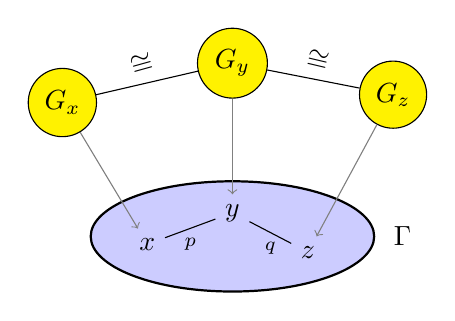
\begin{tikzpicture}[xscale=1.2]
\filldraw[thick, fill=blue, fill opacity=0.2] (0,0) ellipse (1.5 and 0.7);
\node (x) at (-0.9, -0.1) {\(x\)};
\node (y) at (0, 0.3) {\(y\)};
\node (z) at (0.8, -0.2) {\(z\)};
\node at (1.8, 0) {\(\Gamma\)};

\draw (x) edge node[below, font=\scriptsize] {\(p\)} (y);
\draw (y) edge node[below, font=\scriptsize] {\(q\)} (z);

\node[circle, draw=black, fill=yellow] (X) at (-1.8,1.7) {\(G_x\)};
\node[circle, draw=black, fill=yellow] (Y) at (0,2.2) {\(G_y\)};
\node[circle, draw=black, fill=yellow] (Z) at (1.7,1.8) {\(G_z\)};

\draw (X) edge node[sloped, above] {\(\cong\)} (Y);
\draw (Y) edge node[sloped, above] {\(\cong\)} (Z);

\draw[->, gray] (X) -- (x);
\draw[->, gray] (Y) -- (y);
\draw[->, gray] (Z) -- (z);
\end{tikzpicture}
\end{center}

我们可以把 \(\Gamma\) 上的群胚族 \(G_\bullet\) 融为一个
大群胚, 这与 \(\Sigma\)-类型类似, 在范畴论中称为%
\textbf{Grothendieck构造}, 记作 \({\int} G_\bullet\).
具体来说, 它的对象是每个 \(G_x\) 的对象的不交并.
而对于两个元素 \(u \in G_x, v \in G_y\), 它们之间的
道路集合 \(\hom_{{\int} G_\bullet}(u,v)\) 是
\[\{(p, \wp) \mid p \in \hom_G(x,y), \wp \in \hom_{G_y}(G_p(u), v)\}.\]
请读者思考为什么这是唯一自然的选择, 可以参考下面的插图.
\({\int}G_\bullet\) 到 \(\Gamma\) 有明显的群胚同态,
抛弃 \(G\) 的信息.

对于某个群胚族 \(G\), \(\cons{Tm}(G)
= \cons{El}_{F(\Gamma)}(G)\)
则应该是这一族群胚中的“一族元素”. 换句话说, 对每个
\(x \in \Gamma\), 给出群胚 \(G_x\) 中的某个对象
\(g_x\). 对于任何道路 \(p \in \hom(x,y)\), 前面要求的
同构 \(G_p : G_x \to G_y\) 将 \(g_x\) 射到
\(G_p(g_x)\), 我们不能直接要求 \(G_p(g_x) = g_y\),
因为这样过于严格. 但是可以退而求其次, 选择一条道路
\(g_p : G_p(g_x) \to g_y\), 使得
\(g_{\cons{id}} = \cons{id}\), 并且对于连续的两条道路
\(x \xrightarrow p y \xrightarrow q z\), 有
\(g_{p * q} = G_q(g_p) * g_q\). 这实际上就是结合律的要求.

\begin{center}
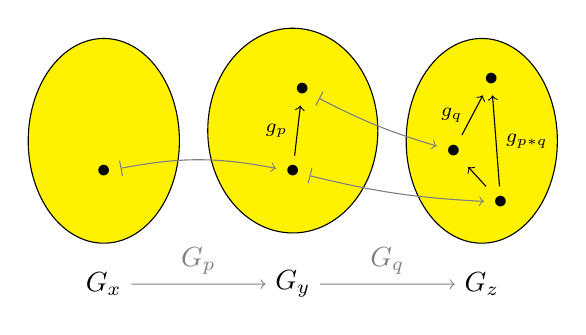
\begin{tikzpicture}[xscale=1.2, yscale=1.3]
\filldraw[fill=yellow] (-2,0) ellipse (0.8 and 1);
\filldraw[fill=yellow] (0,0.1) ellipse (0.9 and 1);
\filldraw[fill=yellow] (2,0) ellipse (0.8 and 1);
\node (Gx) at (-2,-1.4) {\(G_x\)};
\node (Gy) at (0,-1.4) {\(G_y\)};
\node (Gz) at (2,-1.4) {\(G_z\)};
\draw[->, gray] (Gx) edge node [above] {\(G_p\)} (Gy);
\draw[->, gray] (Gy) edge node [above] {\(G_q\)} (Gz);

\node (x) at (-2, -0.3) {\(\bullet\)};
\node (px) at (0, -0.3) {\(\bullet\)};
\node (y) at (0.1, 0.5) {\(\bullet\)};
\node (py) at (1.7, -0.1) {\(\bullet\)};
\node (ppx) at (2.2, -0.6) {\(\bullet\)};
\node (z) at (2.1, 0.6) {\(\bullet\)};

\draw[gray, |->] (x) edge[bend left=10] (px);
\draw[gray, |->] (y) edge[bend right=5] (py);
\draw[gray, |->] (px) edge[bend right=5] (ppx);
\draw[->] (px) edge node[left, font=\scriptsize] {\(g_p\)} (y);
\draw[->] (py) edge node[left, font=\scriptsize] {\(g_q\)} (z);
\draw[->] (ppx) -- (py);
\draw[->] (ppx) edge node[right, font=\scriptsize] {\(g_{p*q}\)} (z);
\end{tikzpicture}
\end{center}

以上就定义了群胚范畴上配备的函子 \(F : \cons{Grpd}\op \to \cons{Fam}\)
在对象上的映射, 我们还需要给出它在态射上的作用. 对于群胚的同态
\(\sigma : \Delta \to \Gamma\), 需要找到集合族的态射
\(\sigma^* : F(\Gamma) \to F(\Delta)\). 在指标集上,
由于 \(\cons{Ix}_{F(\Gamma)}\) 就是 \(\Gamma\) 上的
全体群胚族 \(\Gamma \to \cons{Grpd}\), 因此与 \(\sigma\)
复合就得到
\[(-\circ\sigma) : \cons{Ix}_{F(\Gamma)} \to \cons{Ix}_{F(\Delta)}.\]
而 \(\cons{El}_{F(\Gamma)}(A) \to \cons{El}_{F(\Delta)}(A)\)
的态射也由复合给出.

对于 \(\Gamma\) 与 \(G \in \cons{Ty}(\Gamma)\),
我们最后还需要找到一个对象 \(\Gamma'\) 与态射
\(p : \Gamma' \to G\) 使得
\(\hom_{/\Gamma}(\sigma, p)\) 自然同构于
\(\cons{Tm}(\sigma^*G)\). 只需要取 \(\Gamma'\)
为 \({\int}G_\bullet\) 即可. 这是因为
\((\Gamma, G)\) 在类型论中表现得类似 \(\Sigma\)-类型,
需要将 \(G\) 的所有部分融合. 请读者验证满足条件.

\subsection{群胚族与群胚纤维化}

turn family to fibrations

\subsection{模型范畴} \berryinf

\subsection{无穷范畴}

coherence problem

\section{立方类型论}

泛等公理有很多好的结论, 但是它也有一个问题: 它是一条公理.
而前面已经多次强调过, 如果往类型论中强行加入公理, 就会
破坏它的性质. 这些不好的性质会对形式化数学带来一些困难
------ 尽管不会造成本质性的阻碍, 但是仍然会增加许多工作量.
例如可以在同伦类型论中定义一个自然数, 它不等价于任何一个
具体的自然数, 但是也无法继续化简. (我们仍然可以用相等类型
证明它等于某个具体的自然数, 譬如上文提到的 Brunerie 就
定义了一个自然数为 \(\pi_4(\mathbb S^3)\) 的阶数,
并且证明了这个自然数等于 \(2\). 但是在判值相等关系下
它并不等价于 2.)
有没有办法设计一个类型论, 使得泛等公理成为一个按照
类型规则可以证明的\emph{定理}呢? 答案是肯定的.

我们需要设计一套类型规则, 这是类型论的纯语法操作. 但是,
语法与语义的研究是一体两面的. 此时对同伦类型论的语义研究
推动了新类型规则的设计.

在类型论开始使用\(\infty\)-群胚之前, 拓扑学家已经
对此有了大量的研究. 拓扑学中已经有利用单形(simplex)\footnote{单形就是三角形、四面体等的\(n\)维推广.}
刻画拓扑空间的传统. 我们可以用许多单形拼接成一个拓扑空间,
也可以直接抽象地考虑单形, 将它们看作类似图论或者
组合学的对象处理. 当然, 也有一些使用其他基础形状的研究,
如使用\(n\)维立方体, 或者使用树形等等. 事实上, Daniel Kan
最早的工作就是使用立方体而不是单形. 然而, 这些形状在后续
的研究中发现了它们在一些技术细节上的困难. 因此在拓扑学
研究中\(\infty\)-群胚最常用的还是使用单形的定义.

但是, 对于类型论的研究来说, 基于单形的理论有致命的问题:
它大量使用了排中律和选择公理等非构造性的方法. 2015
年, Bezem与Coquand~\cite{bezem:2015:simplicial}
指出当时的理论中非构造性是无法消除的.%
\footnote{后续研究~\cite{henry:2019:constructive}
中发现可以修改理论去除非构造性. 这与Bezem等人的工作
并不矛盾, 但是这一点的解释超出了本文的范畴.} 我们已经知道
在类型论中, 排中律的各种形式都会或多或少的破坏其性质,
而我们现在的目的就是改善类型论的这些性质, 因此这是不能妥协的.
进一步的研究发现, 基于立方体的理论的技术困难是可以克服的,
并且我们能够建构一套完全构造性的理论. 在 2013 年,
Marc Bezem, Thierry Coquand, Simon Huber 三人提出
用立方集合构建同伦类型论的模型. 在 2017 年他们正式给出了
相关证明~\cite{bch:2017:cubical}. 这套模型由他们的
姓氏首字母称为BCH模型. 根据模型启发了类型论的规则设计,
得到的就是\textbf{立方类型论}.

然而, 这个模型虽然支持泛等公理, 但是由于一些技术原因\footnote{他们
选择的立方体只有最基础的结构, 是由一维的线段直接(在对称张量积下)生成的,
因此没有对角线.}不能支持高阶归纳类型. 在 2017 年,
Cyril Cohen, Thierry Coquand, Simon Huber, Anders M\"ortberg
在论文《立方类型论: 泛等公理的构造性模型》~\cite{abcfhl:2021:cubical}中
四人提出了一个新的模型. 其中立方体的结构由 de Morgan 代数
表示. 根据这个模型(缩写为CCHM模型), 他们构造了一套新的类型论语法. 这
套类型论被称为\textbf{de Morgan立方类型论}.
2019年, Carlo Angiuli等六人提出用区间的Descartes乘积
生成的立方体作为基础, 得到了ABCFHL模型
与\textbf{积立方类型论}.

2021年, Sterling等人发展了范畴论工具, 证明了立方类型论的
典范性. 在他的学位论文~\cite{sterling:2021:thesis}中,
Sterling进一步描述了这些范畴论工具, 并且指出语法与语义研究
之间的关系. 对类型论的范畴语义感兴趣的读者也可以阅读这篇论文.

立方类型论不完全是同伦类型论的子学科. Sterling等人
提出了XTT类型论~\cite{sterling:2019:xtt}, 属于立方类型论,
但是不支持泛等公理等.

\subsection{立方类型论简介}

立方类型论中, 引入了一个类型 \(\mathbb I\) 表示同伦论的区间.
它有两个端点 \(0,1\). 一个变量 \(i : \mathbb I\) 则表示
区间上的一个点. 如果有多个变量, 则它们表示立方体中的某个坐标.
在同伦类型论中, 相等类型的直觉是两点之间道路的空间. 在立方类型论
中, 如果有一条道路 \(p : x =_A y\), 那么就允许我们取出这条
道路上的某一点 \(p(i) : A\). 因此, \(\lambda i. p(i)\) 就是
一个函数 \(\mathbb I \to A\), 而道路空间就可以看成是端点固定的
函数空间.

这样, 我们立刻就可以证明一些定理.

\begin{theorem}
给定函数 \(f : A \to B\), 如果有两个元素 \(x = y\), 那么
\(f(x) = f(y)\).
\end{theorem}
\begin{proof}
我们有 \(p : x = y\). 我们需要证明 \(f(x) = f(y)\).
由于道路空间可以看成端点固定的函数空间, 我们只需要给出一个函数
\(q : \mathbb I \to B\) 使得两个端点 \(q(0) = f(x),
q(1) = f(y)\) 即可. 由于 \(p(i)\) 是道路上的一个点, 有
\(p(i) : A\). 因此 \(f(p(i)) : B\). 我们定义 \(q(i) = f(p(i))\),
验证端点 \(q(0) = f(p(0)) = f(x), q(1) = f(p(1)) = f(y)\)
满足条件.
\end{proof}

\begin{theorem}
如果两个函数逐点相等, 那么它们相等.
\end{theorem}
\begin{proof}
我们有 \(p : \prod_{x : A} f(x) =_B g(x)\). 我们需要证明
\(f =_{A\to B} g\). 由于道路空间可以看成端点固定的函数空间,
我们只需要给出一个函数 \(q : \mathbb I \to (A \to B)\), 使得
两个端点 \(q(0) = f, q(1) = g\) 即可. 我们定义
\(q(i)(x) = p(x)(i)\). 由于 \(p(x) : f(x) =_B g(x)\) 是一条
道路, 因此 \(p(x)(i)\) 就是这条道路上的一个点, 并且其端点符合要求.
\end{proof}

可以看到, 将相等类型使用道路空间的方式定义, 使得证明更加简洁直观.
同时函数外延性在用泛等公理证明时十分复杂, 而使用立方类型论则是最基础的结论.

% 立方类型论版本的闭典范性, 又叫立方闭典范性, 是指将传统意义上的闭典范性中的
% 空语境换成完全由类型 \(\mathbb I\) 拼成的语境
% \(x_1:\mathbb I, x_2:\mathbb I, \cdots, x_n : \mathbb I\).
% 在 2018 年由
% Huber~\cite{huber:2018:canonicity} 提出并证明.

希望继续了解立方类型论的读者可以
参考\href{https://1lab.dev/1Lab.intro.html}{这篇文章}~\cite{amelia:2023:1lab}.
